%%
% Tecnologias Quânticas - MIEF
% Problema 1 - Ordenamento ferrimagnético em magnetite
%
% Data: 24/10/2017


\documentclass[a4paper, 12pt]{article} % Set to article class
\usepackage[portuguese]{babel} % Set language to portuguese

\usepackage{lmodern} % Changes to a cleaner font

\usepackage[T1]{fontenc} % Add support to language
\usepackage[cp1252, utf8]{inputenc} % Add support to language

\chardef\_=`_ % Add support to underscores
\usepackage{graphicx, epstopdf, rotating, % Graphics support
	array, booktabs, float, % Tables packages
	makecell, enumitem, 
	amsmath, amssymb, % Better math print
	siunitx % Plot support	
} % Add basic support

\usepackage[bookmarks, pdftex, hidelinks]{hyperref} % Add hidden bookmarks
\usepackage[margin = .75in]{geometry} % Tool to remove margins
\graphicspath{{images/}} % Add path to images folder

\renewcommand\theadfont{\bfseries} % Make table headers better
\setlength\parindent{0pt} % Remove paragraph indent
\pagestyle{plain} % Adds custom page style
\usepackage[font=small]{caption} % Change caption size

% Nome da disciplina
\def\classtitle{Interação e Deteção de Partículas}

% Nome do relatório
\def\worktitle{Problema 1 - Gerador de Números Aleatórios com uma distribuição exponencial}

% Nome do/a professor/a
\def\profname{Alexandre Lindote}

% Nome do local 
\def\worklocal{Universidade de Coimbra}

% Data do trabalho
\def\workdate{\today}

% Nome dos autores
\def\authors{
	José Nuno da Cruz Faria - 2015252736
}

% Turma
\def\classinfo{Teórica Prática, Turma PL1}

% Resize matrice lines
\makeatletter
\renewcommand*\env@matrix[1][\arraystretch]{%
  \edef\arraystretch{#1}%
  \hskip -\arraycolsep
  \let\@ifnextchar\new@ifnextchar
  \array{*\c@MaxMatrixCols c}}
\makeatother

\begin{document}
	
	\begin{figure}[t] % Add logo
		\centering
		
\includegraphics[width=0.85\linewidth]{uc_fctuc}
	\end{figure}

	\vspace*{0.05\textheight}	
	\begin{table}[!htbp]
		\centering
		
		{\Huge \classtitle}\\
		
		\vspace*{0.01\textheight}
		{\Large \textbf{\worktitle}}\\
		
		\vspace*{0.02\textheight}
		{\large {\worklocal, \workdate}}
		
	\end{table}
	
	\begin{table}[H]
		\begin{center}
			{\normalsize % Mudar a fonte para mais pequena(?)
				\textbf\classinfo\\
				\emph{Prof. \profname}\\ 
				\vspace{0.0035\textheight}			
				\authors 
			}
		\end{center}
	\end{table}

	\section*{Alínea 1)}
	
	O código para o RNG (ficheiro tpc1a.cc) e outros códigos necessários para efetuar compilação encontram-se no link: \url{https://github.com/jncfa/idp_exercices/tree/master/class1/tpc}.

	Para avaliar o gerador RNG, gerámos 2 distribuições com 2 parâmetros diferentes ($\lambda=1$, $\lambda=2$) com $N=10000$ números e efetuamos o seguinte histograma.

	Observou-se uma média de 0.999 para $\lambda=1$ e 0.495 para $\lambda=2$.

	\begin{figure}[H]
		\centering
		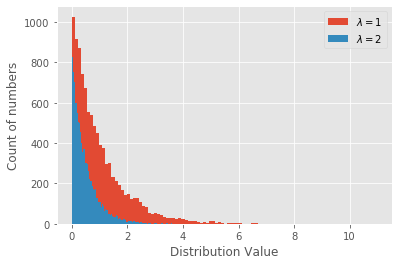
\includegraphics[width=0.8\linewidth]{output.png}
		\caption{Histogramas das distribuições geradas.}
	\end{figure}
\end{document}